\documentclass[jou]{apa6}

\usepackage[american]{babel}

\usepackage{csquotes}
\usepackage[style=apa,sortcites=true,sorting=nyt,backend=biber]{biblatex}
\DeclareLanguageMapping{american}{american-apa}
\addbibresource{bibliography.bib}


%%%%%%%%%%%%%%%%%%%%%%%%%%%%%%%%%%%%%%%%
%% Discrete Structures
%% The start of RBS stuff
%%%%%%%%%%%%%%%%%%%%%%%%%%%%%%%%%%%%%%%%

% Working internal and external links in PDF
\usepackage{hyperref}
% Extra math symbols in LaTeX
\usepackage{amsmath}
\usepackage{gensymb}
\usepackage{amssymb}
% Enumerations with (a), (b), etc.
\usepackage{enumerate}

\let\OLDitemize\itemize
\renewcommand\itemize{\OLDitemize\addtolength{\itemsep}{-6pt}}

\usepackage{etoolbox}
\makeatletter
\preto{\@verbatim}{\topsep=3pt \partopsep=3pt }
\makeatother

% These sizes redefine APA for A4 paper size
\oddsidemargin 0.0in
\evensidemargin 0.0in
\textwidth 6.27in
\headheight 1.0in
\topmargin -24pt
\headheight 12pt
\headsep 12pt
\textheight 9.19in



\title{Sample Quiz 8}
\author{Discrete Structures, Spring 2020}
\affiliation{RBS}

\leftheader{Discrete Sample Quiz 8}

\abstract{%
}

%\keywords{}

\setlength\parindent{0pt}

\begin{document}

%\thispagestyle{empty}

\twocolumn
\section{Worksheet 10: Binary Relations}

\vspace{6pt}
{\bf Question 1 (A reminiscence about variance)}\\
Assume that you want to encode six-letter alphabet 
$\mathcal{A} = \{ \mathtt{a}, \mathtt{b}, \mathtt{c}, \mathtt{d}, \mathtt{e}, \mathtt{f} \}$
and transmit it over a computer network.
You assign $2$ or $3$ bit codes to these letters: 

\begin{tabular}{|l|l|} \hline
{\tt a} & {\tt 00} \\ \hline
{\tt b} & {\tt 01} \\ \hline
{\tt c} & {\tt 100} \\ \hline
{\tt d} & {\tt 101} \\ \hline
{\tt e} & {\tt 110} \\ \hline
{\tt f} & {\tt 111} \\ \hline
\end{tabular}

For example, the 11-bit sequence {\tt "10100100110"} means {\tt "dace"}.
Denote by $X$ the random variable \textendash{} the number of 
bits used to encode a single letter. (All $6$ letters have 
equal probabilities.)

Find $E(X)$ and $V(X)$.\\
Write them as two fractions: {\tt P1/Q1,P2/Q2}\\
(Separate the fractions by comma, 
do not leave any spaces.)


\vspace{6pt}
{\bf Question 2 (Rosen7e, Ch.9, Q10-Q23).}\\
Determine whether the binary relation is: (1) reflexive, (2) symmetric, (3) antisymmetric, (4) transitive.
Express your answer as as a 4-letter string of T/F (true/false values that are 
answer to these $4$ questions). For example, {\tt TFTT} etc.
%For example, the relationship $a \leq b$ on $\mathbb{Z}$ has these answers: {\tt TFTT}. It is reflexive, antisymmetric
%and transitive. But $\leq$ is not symmetric ($a \leq b$ does not imply that $b \leq a$).
\begin{enumerate}[(A)]
\item The relation $R$ on $\{1, 2, 3,\ldots\}$ where $aRb$ means $a\,\mid\,b$.
\item The relation $R$ on $\{w, x, y, z\}$ where $R = \{(w, w), (w, x), (x, w), (x, x), (x, z), (y, y), (z, y), (z, z)\}$.
\item The relation $R$ on $\mathbb{Z}$ where $aRb$ means $|a - b| \leq 1$.
\item The relation $R$ on $\mathbb{Z}$ where $aRb$ means $a \neq b$.
\item The relation $R$ on $\mathbb{Z}$ where $aRb$ means that the units digit of $a$ is equal to the units digit of $b$.
\item The relation $R$ on the set of all subsets of $\{1, 2, 3, 4\}$ where $SRT$ means $S \subseteq T$.
\item The relation $R$ on the set of all people where $aRb$ means that a is younger than $b$.
\item The relation $R$ on the set $\{(a, b) \,\mid\, a, b \in \mathbb{Z}\}$ where $(a, b)R (c, d)$ means $a = c$ or $b = d$.
\end{enumerate}

\vspace{6pt}
{\bf Question 3 (Rosen7e, Ch.9, Q35-Q38).}\\
Construct a matrix of the relations defined below. Output the matrix as a list of lists:\\
{\tt [[a11,a12,...],[a21,a22,...],...]}
\begin{enumerate}[(A)]
\item $R$ on $\{1, 2, 3, 4, 6, 12\}$ where $aRb$ means $a\,\mid\,b$.
\item $R$ on $\{1, 2, 3, 4, 6, 12\}$ where $aRb$ means $a \leq b$.
\item $R^2$, where $R$ is the relation on $\{1, 2, 3, 4\}$ such that $aRb$ 
means $|a - b| \leq 1$.
\end{enumerate}

\vspace{6pt}
{\bf Question 4 (Rosen7e, Ch.9, Q42).}\\
Define
$$M_R = \left( \begin{array}{cccc}
1 & 0 & 1 & 0 \\
1 & 0 & 0 & 1 \\
1 & 1 & 1 & 0 \\
1 & 1 & 0 & 1 \\
\end{array} \right)$$
determine if $R$ is: (1) reflexive (2) symmetric (3) antisymmetric (4) transitive.
Express your answer as as a 4-letter string of T/F (true/false values that are 
answer to these $4$ questions). For example, 
{\tt TFTT} etc.


\vspace{6pt}
{\bf Question 5 (Rosen7e, Ch.9, Q47).}\\
Let $A$ be the set of all positive divisors of $60$ (including $1$ and $60$ itself). 
Draw the Hasse diagram for the relation $R$ on $A$ where $aRb$ means $a\,\mid\,b$.

\vspace{6pt}
{\bf Question 6 (Rosen7e, Ch.9, Q51).}\\
Find the transitive closure of $R$ if 
$$M_R  = \left( \begin{array}{cccc}
1 & 0 & 1 & 0 \\
1 & 0 & 0 & 1 \\
0 & 1 & 1 & 0 \\
0 & 1 & 0 & 0 \\
\end{array} \right).$$

\vspace{6pt}
{\bf Question 7 (Rosen7e, Ch.9, Q59).}\\
Find the join of the 3-ary relation:
\begin{verbatim}
{ (Wages,MS410,N507),
  (Rosen,CS540,N525),
  (Michaels,CS518,N504),
  (Michaels,MS410,N510) }
\end{verbatim}
and the 4-ary relation:
\begin{verbatim}
{ (MS410,N507,Monday,6:00), 
  (MS410,N507,Wednesday,6:00), 
  (CS540,N525,Monday,7:30),
  (CS518,N504,Tuesday,6:00), 
  (CS518,N504,Thursday,6:00) }
\end{verbatim}
with respect to the last two fields of the first relation and 
the first two fields of the second relation. 

\vspace{6pt}
{\bf Question 8 (Rosen7e, Ch.9, Q69-Q71).}
Give an example of a relation or state that there are none.\\
{\bf (A)} A relation on $\{a, b, c\}$ that is reflexive and transitive, but not antisymmetric.\\
{\bf (B)} A relation on $\{1, 2\}$ that is symmetric and transitive, but not reflexive.\\
{\bf (C)} A relation on $\{1, 2, 3\}$ that is reflexive and transitive, but not symmetric.

\vspace{6pt}
{\bf Question 9 (Rosen7e, Ch.9, Q73).}\\
Suppose $|A| = 7$. Find the number of reflexive, symmetric binary relations on $A$.





\newpage

\subsection{Answers}


\vspace{6pt}
{\bf Question 1.} 
The random variable $X$ takes value $x_1 = 2$ (with probability $p_1 = \frac{1}{3}$)
and value $x_2 = 3$ (with probability $p_2 = \frac{2}{3}$). 
We can compute: 
$$E(X) = x_1p_1 + x_2p_2 = \frac{8}{3}.$$
$$V(X) = (x_1 - E(X))^2p_1 + (x_2 - E(X))^2p_2 = \frac{2}{9}.$$

\vspace{6pt}
{\bf Question 2.} 
\begin{enumerate}[(A)]
\item {\tt TFTT}
\item {\tt TFFF}
\item {\tt TTFF}
\item {\tt FTFF}
\item {\tt TTFT}
\item {\tt TFTT}
\item {\tt FFTT}
\item {\tt TTFF}
\end{enumerate}

\vspace{6pt}
{\bf Question 3.}\\
{\bf (A)} Divisibility on the set $\{1, 2, 3, 4, 6, 12\}$
$$M_R  = \left( \begin{array}{cccccc}
1 & 1 & 1 & 1 & 1 & 1 \\
0 & 1 & 0 & 1 & 1 & 1 \\
0 & 0 & 1 & 0 & 1 & 1 \\
0 & 0 & 0 & 1 & 0 & 1 \\
0 & 0 & 0 & 0 & 1 & 1 \\
0 & 0 & 0 & 0 & 0 & 1 \\
\end{array} \right).$$
{\bf (B)} Relation $\leq$ on the set $\{1, 2, 3, 4, 6, 12\}$
$$M_R  = \left( \begin{array}{cccccc}
1 & 1 & 1 & 1 & 1 & 1 \\
0 & 1 & 1 & 1 & 1 & 1 \\
0 & 0 & 1 & 1 & 1 & 1 \\
0 & 0 & 0 & 1 & 1 & 1 \\
0 & 0 & 0 & 0 & 1 & 1 \\
0 & 0 & 0 & 0 & 0 & 1 \\
\end{array} \right).$$
{\bf (C)} Relation $R^2$, where $aRb$ iff $|a-b| \leq 1$.
$$M_R  = \left( \begin{array}{cccc}
1 & 1 & 1 & 0 \\
1 & 1 & 1 & 1 \\
1 & 1 & 1 & 1 \\
0 & 1 & 1 & 1 \\
\end{array} \right).$$
The only pairs that do not belong to $R^2$ are 
$(1;4)$ and $(4;1)$. 




\vspace{6pt}
{\bf Question 4.} Answer: {\tt FFFF}\\
Imagine that the relation $R$ is defined on a set of these 4 elements:
$a,b,c,d$. 
\begin{itemize}
\item $R$ is not reflexive, since $bRb$ is false (the matrix has $m_{22}=0$).
\item $R$ is not symmetric, since $bRa$ does not imply $aRb$
(the matrix has $m_{12}=0$, but $m_{21}=1$).
\item $R$ is not antisymmetric, since $aRc$ and $cRa$ both hold, but 
$a \neq c$.
\item $R$ is not transitive, since $aRc$ and $cRb$, but $aRb$ is not true.
\end{itemize}

\vspace{6pt}
{\bf Question 5}:\\
Hasse diagram connects only those numbers $a,b$ where $a$ divides $b$, and
there is no third  number in-between (such that $a\,\mid\,c$ and $c\,\mid\,b$). 
For example, $1$ and $2$ are connected, but $1$ and $4$ are not 
(because the relation $1\,\mid\,4$ can be inferred from 
$1\,\mid\,2$ and $2\,\mid\,4$).
\begin{center}
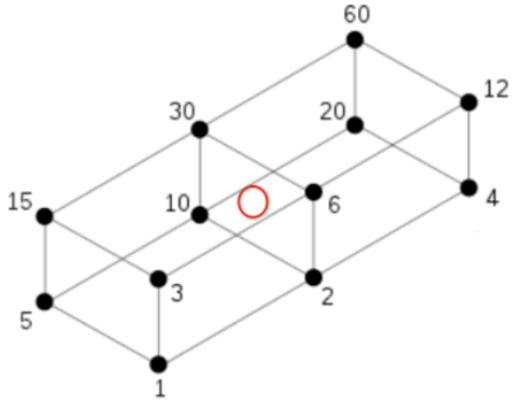
\includegraphics[width=2.5in]{hasse-diagram-60.png}
\end{center}
Note that the Hasse diagram for divisibility is centrally symmetric. 
(This is true for any set of divisors for some number.)


\vspace{6pt}
{\bf Question 6}:\\
$$M_R  = \left( \begin{array}{cccc}
1 & 0 & 1 & 0 \\
1 & 0 & 0 & 1 \\
0 & 1 & 1 & 0 \\
0 & 1 & 0 & 0 \\
\end{array} \right).$$

Denote the elements of the set by $a,b,c,d$. We want to find, 
what are the ``relational paths'' between them:
\begin{itemize}
\item Path $aRc$, $cRb$, $bRd$ adds $(a,b)$, $(a,d)$ to the transitive closure.
\item Path $bRa$, $aRc$, $cRb$ adds $(b,c)$, $(b,b)$ to the transitive closure.
\item Path $cRb$, $bRd$ adds $(c,d)$ to the transitive closure.
\item Path $cRb$, $bRa$ adds $(c,a)$ to the transitive closure.
\item Path $dRb$, $bRa$, $aRc$ adds $(d,a)$, $(d,c)$.
\item Path $dRb$, $bRd$ adds $(d,d)$.
\end{itemize}

Here is the matrix 
of the transitive closure after all the new pairs are added:

$$M_{R\ast}  = \left( \begin{array}{cccc}
1 & 1 & 1 & 1 \\
1 & 1 & 1 & 1 \\
1 & 1 & 1 & 1 \\
1 & 1 & 1 & 1 \\
\end{array} \right).$$



\vspace{6pt}
{\bf Question 7}\\
TBD (see Section 9.2.4 of the textbook (Definition 4, page 615)). This problem 
is based entirely on applying the definition.

\vspace{6pt}
{\bf Question 8}\\
{\bf (A)} TBD\\
{\bf (B)}. Yes. We can have a relation $R$ which is 
never satisfied. It is symmetric and also transitive
(since $xRy$ and $yRz$ can never happen, so we do not
need to care about $xRz$).\\
{\bf (C)}. TBD.


\vspace{6pt}
{\bf Question 9} Answer: {\tt 2097152}\\
The matrix $M$ of any relation $R$ on a set of $7$ elements has $49$ entries. 
The entries on the main diagonal ($m_{11},m_{22},\ldots,m_{77}$) 
should all equal $1$ ($R$ is reflexive). 
Also, any entry $m_{ij}$ above the main diagonal ($i<j$ - row number is
less than the column number) is symmetric to some entry below the diagonal
$m_{ji}$ (where $i>j$). 

Therefore we can freely choose only those $m_{ij}$ that are above the main 
diagonal; everything else is predetermined. There are $1+2+\ldots+6=21$ such 
elements in the matrix. The total number of ways to choose them is
$2^{21} = 2097152$.




\end{document}

